\documentclass[12pt, oneside]{article}

\usepackage{graphicx}
\usepackage{hyperref}
\graphicspath{{images/}}

\begin{document}

\section{Functional Requirements}

\subsection{System Features}

\subsubsection{Functions To Apply Social Tagging}
\begin{itemize}
\item The system will provide functions which through employing tags can provide flexible ways of using information that supports users with: Finding, Collecting, Storing, Organizing and Sharing Information.
\item Allow users to share their tags.
\item Allow users different views of the content. Either a personally structured view according to the user's tags or the default admin structure.
\end{itemize}

\subsubsection{Apply Self-Organization}
\begin{itemize}
\item The system will allow the user to organize their content themselves based on their social tags.
\item The system will allow the user to chose from different types of views either the base owns or public structure.
\end{itemize}
\subsection{Pre-conditions}
\subsubsection{Social Tagging Functions}    
\begin{itemize}
\item User is signed in and has default privileges to execute all social tagging functions functions.
\item User has already created tags before they can share them.
\item  System allows for different views of the content.
\end{itemize}
\subsubsection{Self-Organization Based On Social Tagging}
\begin{itemize}
\item Have three different structures users can choose from for viewing.
\end{itemize}

\subsection{Post-conditions}
\subsubsection{Social Tagging Functions}    
\begin{itemize}
\item After the user has executed any of the functions the user state changes.
\item After the user selects their view structure, the structure must stay consistent until the user chooses otherwise.
\end{itemize}
\subsubsection{Self-Organization Based On Social Tagging}
\begin{itemize}
\item After the user selects their view type, provide option to still be able to switch views.
\item Content must be displayed according to user's desire.
\end{itemize}
\section{Use Cases}
  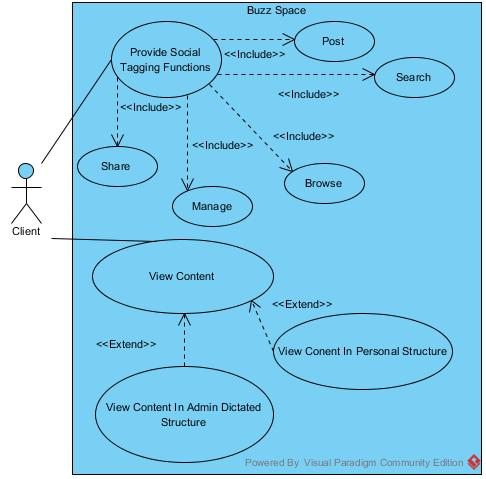
\includegraphics{u29630135_socialTagging.jpg}
    \rule{0\linewidth}{0.15\linewidth}\par
\end{document}